% Created 2024-10-16 śro 21:35
% Intended LaTeX compiler: pdflatex
\documentclass[../../main.tex]{subfiles}

% \usepackage[a4paper, margin=3cm]{geometry}
% \usepackage{amssymb} // not working

\usepackage[T1]{fontenc}
\usepackage[utf8]{inputenc}
\usepackage{graphicx}
\usepackage{longtable}
\usepackage{wrapfig}
\usepackage{rotating}
\usepackage[normalem]{ulem}
\usepackage{amsmath}
\usepackage{capt-of}
\usepackage{hyperref}
\usepackage{siunitx}
\usepackage{float}
\usepackage[polish]{babel}

\graphicspath{{../}}
\author{Wojciech Paderewski}
\date{\today}
\title{LDO}
\hypersetup{
 pdfauthor={Wojciech Paderewski},
 pdftitle={LDO},
 pdfkeywords={},
 pdfsubject={},
 pdflang={Polish}}
\begin{document}

Wybrano horyzontalne złącze gold pin, ponieważ łatwo jest podłączyć do niego uniwersalne przewody żeńskie, często wykorzystywane w prototypowaniu.
Horyzontalna wersja złącza została wybrana, by nie zwiększać wysokości płytki. Dodatkową zaletą tego rozwiązania jest ewentualna możliwość programowania
mikrokontrolera za pomocą tego złącza w przypadku, gdyby nie udało się tego zrobić przez USB. 

Złącze będzie wystawiać następujące sygnały:
\begin{itemize}
    \item RX - odbiór danych
    \item TX - wysyłanie danych
    \item GND - masa
\end{itemize}

W celu zabezpieczenia złącza przed ESD zastosowano transil, analogiczny jak w podrozdziale \ref{sec:usb_c_to_program}.
Schemat złącza przedstawiono na rysunku \ref{fig:uart}.

\begin{figure}[H]
    \centering
    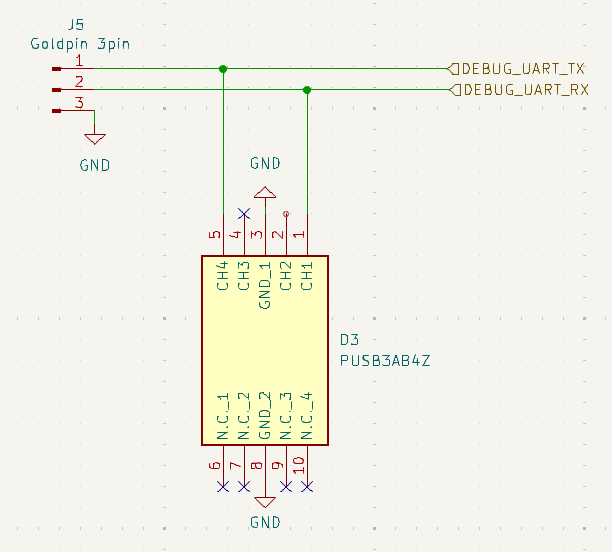
\includegraphics[width=0.8\textwidth]{uart.png}
    \caption{Schemat elektryczny złącza UART}
    \label{fig:uart}
\end{figure}

\end{document}
